\chapter{Simulator}
\label{chap:sim}

\begin{figure}
	\centering
	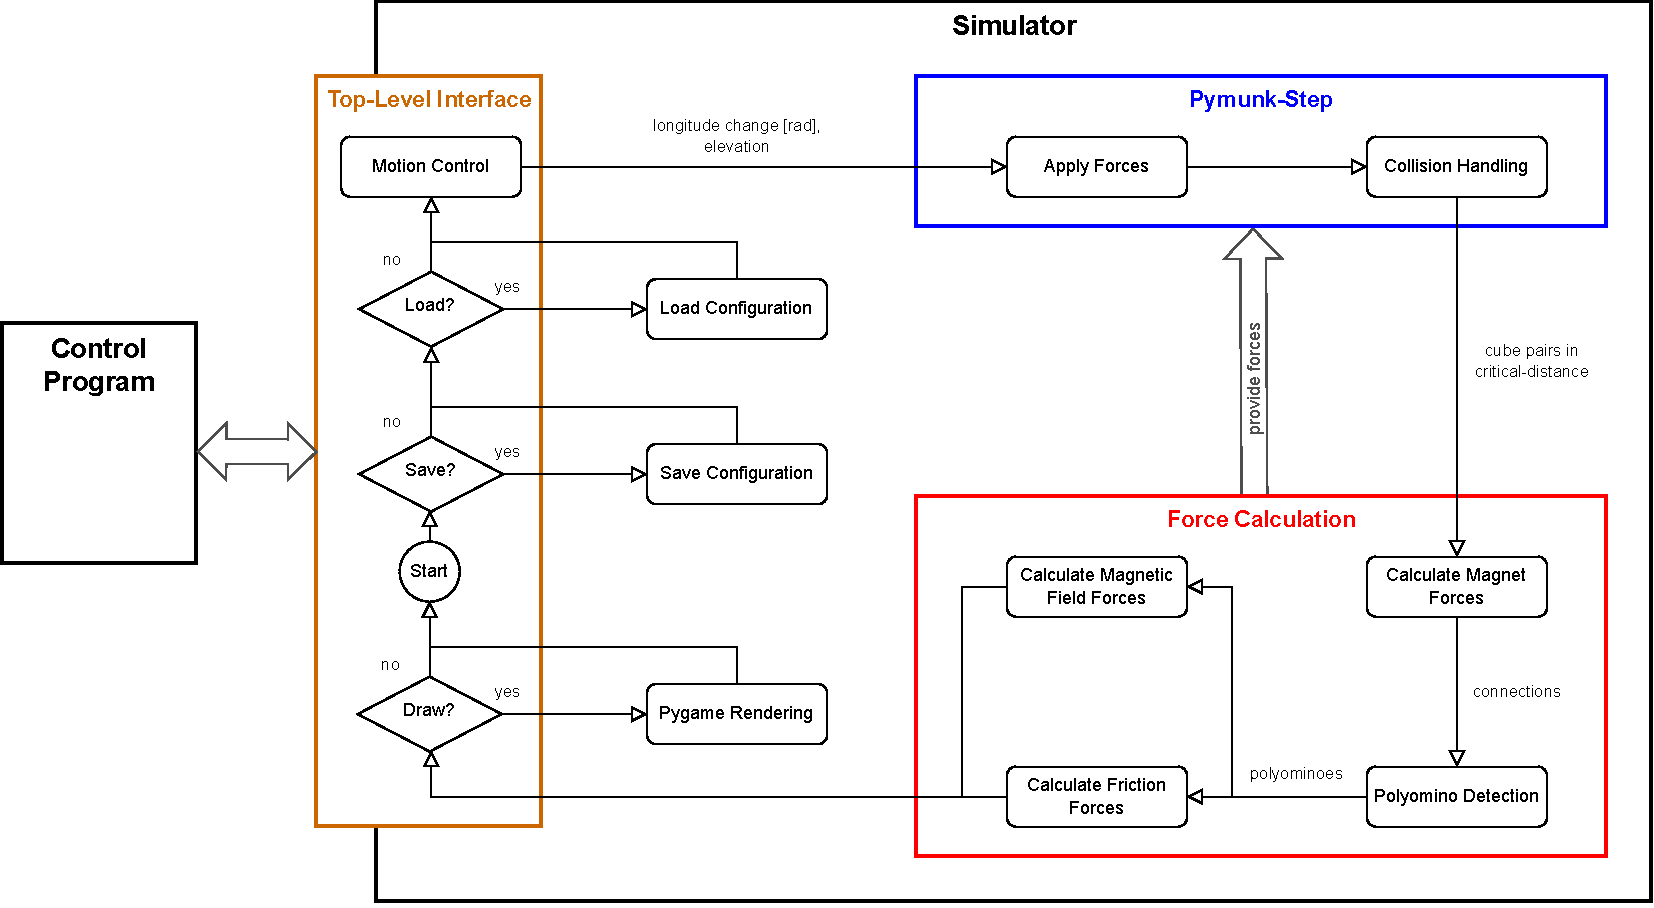
\includegraphics[width=1\textwidth]{figures/simulator_controlflow.pdf}
	\caption[Control flow of the simulator]{Flow chart diagram illustrating the control flow of the simulators simulation loop. Any control program can interact with the top-level interface of the simulator. Further Tasks are grouped in the Pymunk-step and the force calculation. Calculated forces are provided to the Pymunk-step for the next iteration of the loop.}
	\label{fig:simulator}
\end{figure}

\begin{figure}
	\centering
	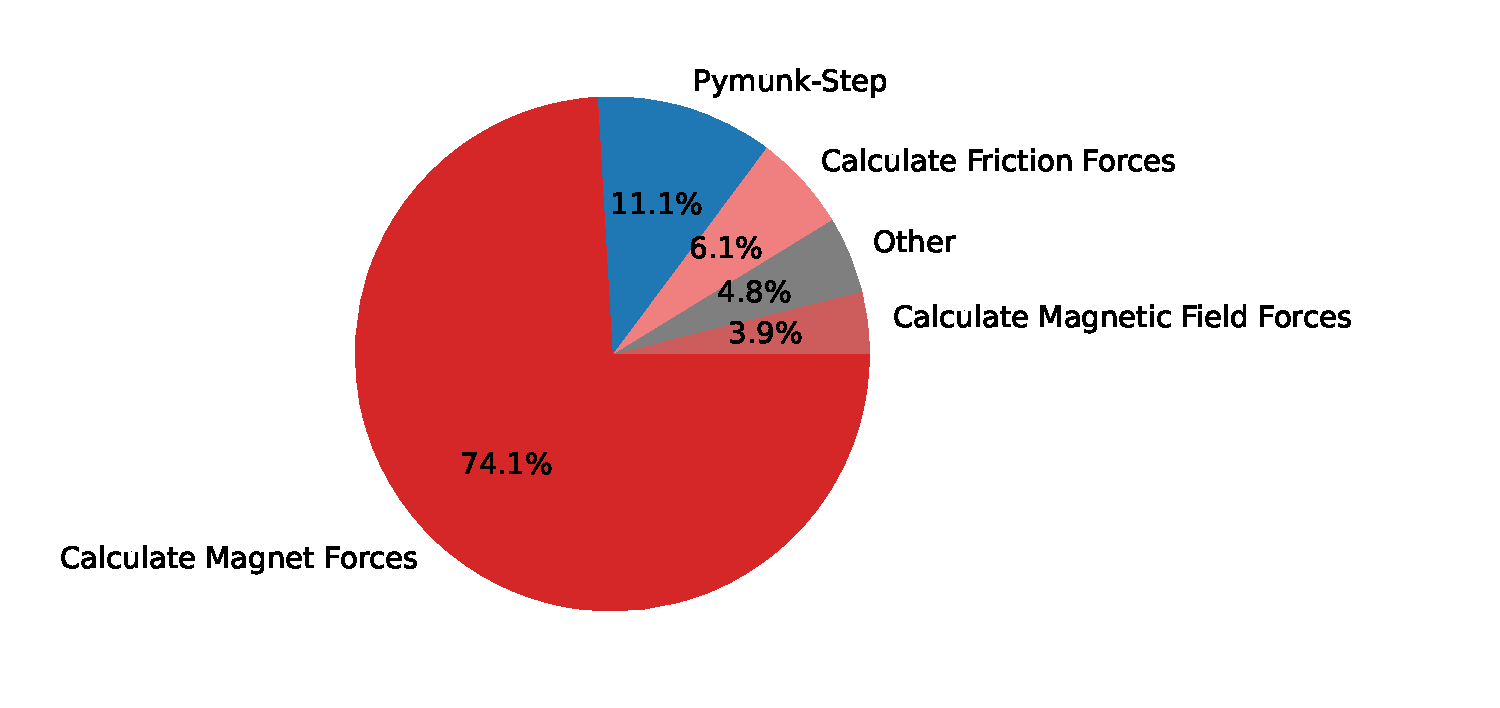
\includegraphics[width=0.9\textwidth]{figures/plots/simulator_timeuse.pdf}
	\caption[Diagram of time-use for certain steps in simulation loop]{Fraction of time used on certain steps in the simulation loop. The simulator ran for $8$ seconds without drawing and executed various motions with ten cubes in the workspace. The steps can be found in the control flow illustrated in \autoref{fig:simulator}}
	\label{fig:timeuse}
\end{figure}

Our simulator used for modeling the behavior of magnetic modular cubes uses the 2d physics library Pymunk\footnote{Pymunk: \url{https://www.pymunk.org/}}.
This library is build for the Python 3 and Python 2 environment based on the 2d physics library Chipmunk\footnote{Chipmunk: \url{http://chipmunk-physics.net/}}.
We used Pymunk, since it can be easily integrated and customized in a Python implementation.
Furthermore it is light-weight and capable of running headless, but also offers an interface for Pygame\footnote{Pygame: \url{https://www.pygame.org/}}, which we use to visualize developed plans and to allow user controls.
As a disadvantage, we are challenge with the simulation of 3d movement in a 2d environment.
This way we trade simulation accuracy for faster simulation time, which is necessary to develop global plans in a reasonable time.

In \autoref{fig:simulator} a flow chart diagram illustrates the control flow of the simulators simulation loop.
The individual steps in the diagram are explained in this and in the following sections.

Any control program, for example a local planner or a ``sandbox program'' for visually controlling magnetic modular cubes with keyboard inputs, can interact with the top-level interface of the simulator.
The interface provides functionalities like starting and stopping the simulation process, controlling the drawing with Pygame, or loading custom configurations and retrieving the current workspace state (\autoref{sec:workspace_state}).
Another crucial functionality is queuing in motions for simulation and notifying the control program when a motion is done simulating.
After handling the motion control, further explained in \autoref{sec:motion_control}, the simulator enters the Pymunk-step.

The Pymunk-step is a library function, responsible for updating the simulation environment by a certain time step.
The duration of a time step is a parameter that allows adjustment between simulation accuracy and simulation time. 
Inside the Pymunk-step forces are applied to the cubes and collision with workspace boundaries and between cubes is handled (\autoref{sec:coll_handling}).

After the Pymunk-step the magnetic forces between the cubes permanent magnets are calculated.
This also determines connections of cube faces that will be used to retrieve information about polyominoes in the workspace (\autoref{sec:force_magnet}).
Polyomino information is necessary to calculate forces of the magnetic field acting on cubes (\autoref{sec:force_field}) and friction forces, on which we heavily rely to simulate 3d movement like pivoting on pivot edges (\autoref{sec:force_friction}).
All the calculated forces will be applied in the Pymunk-step next iteration.

When drawing is enabled, the Pygame-rendering of the workspace is the last step before beginning the next iteration.

% plot of time use for simulation

\section{Motion Control}
\label{sec:motion_control}

The motion control manages the queued-in motions from the control program and determines a change of the magnetic field for each iteration of the simulation loop.
This change consists of the longitude change in radians and the latitude change called the elevation.
In our simulator the elevation states if the magnetic field lays in the workspace plane or if the magnetic north or south is pointing up.
We do not specify an angular value of the latitude.
The elevation just indicates if polyominoes are pivoting or not.
More on that in \autoref{sec:force_friction}.

A change of elevation is executed in a single iteration, but the angle of a rotation will be simulated by multiple longitude changes in a linear ramp with a rotational velocity we choose to set to $\frac{\pi}{8} \, \text{rad}/\text{s}$.
Each motion will be simulated by applying its sequence of updates with a notification to the control program when done.
This makes closed loop control possible, by letting the control program wait until motions are simulated.

Motions control the magnetic field orientation and not the cubes directly.
Cubes will orient themselves by magnetic field forces we further explain in \autoref{sec:force_field}.
The larger a polyomino is, the more time it needs to align with the magnetic field, which can take longer than rotating the magnetic field itself.
A certain amount of zero-updates, dependent on the size of the larges polyomino in the workspace, is added to a rotations update sequence.
This way the control program will not be notified until all polyominoes are aligned with the magnetic field.
This is the reason simulating larger polyominoes requires more simulation time.

\section{Workspace State}
\label{sec:workspace_state}

The state of the workspace is stored and updated within the Pymunk-space.
By saving a configuration of the workspace, relevant attributes like position, orientation and velocity of cubes are copied from the Pymunk-space.
When loading in a configuration, the attributes of the Pymunk-space will be manipulated.

Furthermore a configuration stores magnetic field orientation and the polyominoes, together with their center of mass and pivot points.
Polyominoes are stored in a custom data structure that functions both as a list of physical polyominoes and a polyomino set for the use in two-cut-sub-assembly graphs (\autoref{sec:tcsa}).
The data structure and the polyominoes themselves are hash-able for fast equality and inclusion checks.

Individual orientation and velocities of cubes will not be used for planning, but they ensure a correct loading of a workspace configuration that got saved while in motion or when cubes where not or not yet aligned with the magnetic field.
The alignment can be prevented by walls or other cubes, even though we assume perfect alignment with the magnetic field during planning.

\begin{figure}
	\centering
	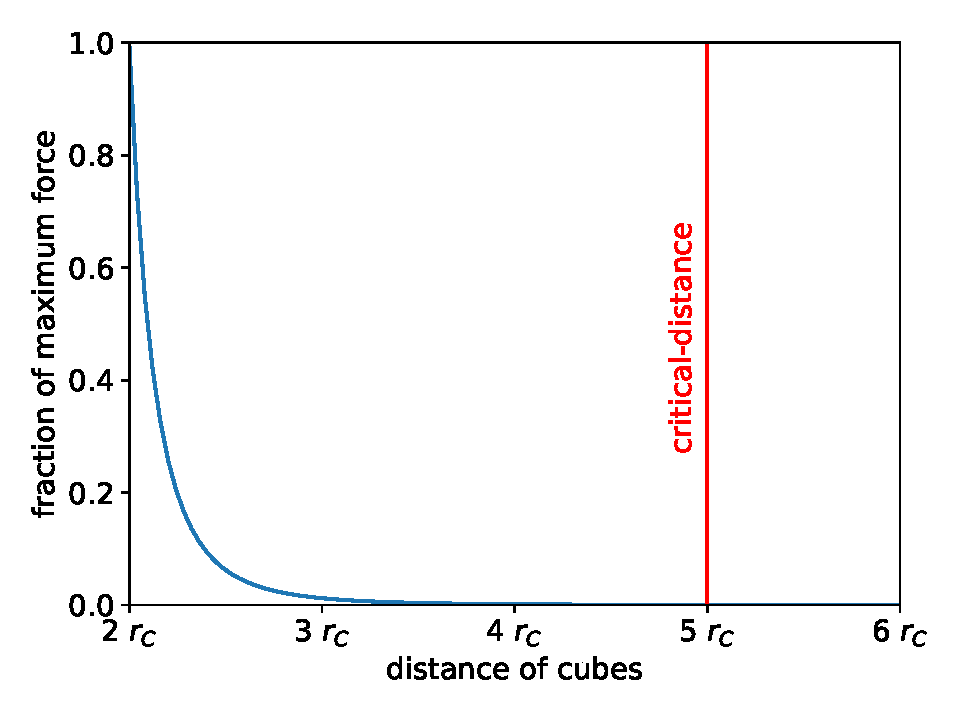
\includegraphics[width=0.6\textwidth]{figures/plots/magnet_force.pdf}
	\caption[Declining magnetic forces with increasing cube distance.]{Decline of magnetic force between two permanent magnets with increasing distance between the cubes. We reach a maximum force at $2 r_C$, when the cube faces are connected. With distances bigger than the critical-distance of $5 r_C$ the fraction of force is negligible.}
	\label{fig:magnet_force}
\end{figure}

\section{Collision Handling}
\label{sec:coll_handling}

Collision is detected and resolved by Pymunk during the Pymunk-step.
For the collision detection Pymunk uses a bounding volume hierarchy of objects in the Pymunk-space.
We make use of this efficient collision detection for determining cube pairs in critical-distance.
For that, each cube is surrounded by a circular sensor with a radius of half the critical-distance.
A cube pair is in critical-distance if their sensors collide.
Cubes not in critical-distance are to far away to significantly affect each other with magnetic forces of their permanent magnets.
We only calculate magnet forces for cube pairs in critical-distance to speed up simulation.
The critical-distance is $5 r_C$ and illustrated in \autoref{fig:magnet_force} together with the decline of magnetic force with increasing cube distance.

\section{Simulating Forces}

\cite{Lu2023}

% apply with pymunk

\subsection{Magnet Forces}
\label{sec:force_magnet}

% pull cubes together
% provide equation
% hold cubes together -> polyomino detection
% wich magnetic pairs to choose
% minDist, minDists, all

\subsection{Magnetic Field Forces}
\label{sec:force_field}

% applied to top bottom each indivial cube
% as long as orientation doenst match
% the bigger the poly the longer rotations actually take 
% adding zero updates to motion so that motion finishes when polys oriented


\subsection{Friction Forces}
\label{sec:force_friction}

% force to let poly rotate around pivot point
% splitt friction on cubes on pivot edge
% nominal friction to prevent breaking


